\section{Evaluation}
\label{sec:eval}

We evaluate \sdr on its merits as a low-power SDR platform. Specifically, we
focus on its power consumption, latency, and hardware flexibility. We further
examine the performance of the \sdr system in the exploration of the low-power
802.15.4 MAC protocol.

\vfill\eject

\subsection{Platform Micro-Benchmarks}
Designing a low-power system requires building from the ground up with
low-power components. In traditional software radio designs, one of the
largest power sinks is the FPGA. The recent influx of flash-based FPGAs open
the door to low power design. In Table~\ref{tab:fpga_static_current} we
compare the static power draw of the flash-based SmartFusion to the SRAM-based
Xilinx Spartan~3-2000 used in the USRP 2. The superior FPGA core power
efficiency of the flash-based FPGA is a direct consequence of the technology.
Freed of the requirement to continually refresh the logic cells, the flash
FPGA consumes very little static power. As a young technology, we expect these
innovations in static power for flash-based FPGAs to improve rapidly, as
evidenced by the Microsemi IGLOO series, whose Flash*Freeze technology lowers
the FPGA static power draw as far as 2~uW~\cite{igloo}.

In addition to the impact on static power usage, flash-based FPGAs also excel
during cold-boot. For an FPGA to be useful, it must at some point be
configured. In the case of SRAM-based FPGAs, this configuration must occur at
every boot, as the configuration of the FPGA is lost when power is no longer
supplied. This configuration period introduces a non-trivial delay for the
FPGA wake-up process as well as consuming a relatively large amount of power.
Most importantly, the latency imposed by the configuration window inhibits
effective duty-cycling of the FPGA. In Figure~\ref{fig:coldboot}, we compare
the cold boot times of the SRAM-based USRP 2 (\ref{fig:usrp_coldboot}) to the
\sdr (\ref{fig:usdr_coldboot}). After a system in-rush current spike of
1.8~A, the USRP 2 averages a 700~mA current draw for 1.964~s while it
configures its FPGA. This long configuration process and high current
consumption consume 9.56~J of energy, a cost that must be paid every time the
FPGA is power cycled.

\begin{table}
	\centering
	\begin{tabular}{|c|c|c|}
		\hline
		\rowcolor[gray]{0}
		 % first column blank
		 & {\sc {\color{white} SmartFusion}}
		 & {\sc {\color{white} Spartan}} \\ 
		\rowcolor[gray]{0}
		  {\sc {\color{white} voltage rail}}
		& {\sc {\color{white} static current}}
		& {\sc {\color{white} static current}} \\ \hline
		3.3V (IOs )	& 85.6 mA 	& 79 mA \\ \hline
		2.5V (Aux) 	& n/a		& 88 mA \\ \hline
		1.5V (Core)	& 7.76 mA 	& n/a   \\ \hline
		1.2V (Core)	& n/a		& 80 mA \\ \hline
		\rowcolor[gray]{.9}
		Total Power	& 294 mW	& 578 mW \\ \hline
	\end{tabular}
    \caption{Static current at each supply rail for the SmartFusion and
In contrast, \sdr has no current spike on bootup and an average current
consumption of under 100~mA. To measure time to first useful instruction, we
wrote a simple program that simply toggles an IO line, indicating the
processor is ready to start executing. We measured the time from power
application until the IO asserts. The \sdr requires 259~ms to boot the system,
consuming only 0.101~J. Even the latency of \sdr is not ideal for a rapid
duty cycled system, which would ideally be in the {\em microsecond} range as
opposed to {\em milliseconds}. \sdr is remains significantly better than the
USRP 2's {\em seconds} to boot: $7.6\times$ faster in terms of latency and
$94.7\times$ lower in terms of energy consumption.
platforms.}
	\label{tab:fpga_static_current}
\end{table}

\begin{figure*}[t]
	\centering
    \subfigure[USRP2 Cold Boot]{
        \includegraphics[width=0.45\textwidth]{usrp_coldboot/usrp_coldboot}
        \label{fig:usrp_coldboot}
    }
    \subfigure[\sdr Cold Boot]{
        \includegraphics[width=0.45\textwidth]{usdr_coldboot/usdr_coldboot}
        \label{fig:usdr_coldboot}
    }
    \caption{USRP2 and \sdr cold boot comparison. Both systems power on at
{\em 0~s}. As expected, the USRP2 \subref{fig:usrp_coldboot} has a current
spike of 1.8~A, and exhibits an average current draw of 700~mA at 6~V. It
takes 1.96~s to load the firmware from an external SD card, resulting in
9.56~Joules of energy consumption during cold boot. In contrast, the
flash-based \sdr doesn't have an in-rush current and the average current is
less than 100~mA at 3.3~V. Moreover, \sdr requires 259~ms to boot the system,
resulting in only 0.101~Joules of energy consumption. \sdr is 7.6$\times$
faster and uses 100$\times$ less energy than the USRP2 to start-up.}
\label{fig:coldboot}
\end{figure*}

Given that the 259~ms boot time is too highly latent to support aggressive
duty-cycling, \sdr also presents a sleep mode as a median option between
system full on and full off. Unfortunately, the SmartFusion chip is only
capable of sleeping the M3 core (via WFI\footnote{WFI: Wait For Interrupt, and
ARM instruction that places the core in a lower power sleep state until
interrupted. The contents of registers are preserved but the rest of the core
is power gated}). Fully sleeping the FPGA would require technology similar to
the Flash*Freeze mode from the Microsemi IGLOO line of low-power FPGAs.
Unfortunately these FPGAs do not yet support the tight integration with a hard
CPU and are currently unsuitable for the \sdr platform. Until technology
similar to Flash*Freeze comes to the SmartFusion, \sdr is still capable of
lowering the FPGA power via frequency scaling. In \sdr's frequency scaling
mode we turn off the external crystal oscillator and used the FPGA's internal
RC network instead. The frequency of the RC network is reduced to 6.5\% of
the original frequency (to 3.125~MHz). We additionally turned off the PLL and
bypassed two other clock sources for FPGA logic to further reduce the system
current. Table~\ref{tab:sdr_wfi_duty_cycle} examines the impact of these power
saving efforts. Simply placing the processor in WFI state and power gating all
external components reduces system power consumption to 108~mA with only
34~$\mu$s of wakeup latency. Introducing FPGA frequency scaling reduces
system power further to 67~mA, but imposes a 3.01~ms latency to turn on the
crystal oscillator and stabilize the PLL until the processor can be woken.

\begin{table}[h]
	\centering
	\begin{tabular}{ | c | c | c | }
		\hline
		\rowcolor[gray]{0}
		  {\sc {\color{white} Frequency}}
		& {\sc {\color{white} Wake-up}}
		& {\sc {\color{white} System}}
		\\
		\rowcolor[gray]{0}
		  {\sc {\color{white} Scaling}}
		& {\sc {\color{white} Latency}}
		& {\sc {\color{white} Power}}
		\\ \hline
% 108mA * 4.8 , 67 * 4.8
		off	& 34 $\mu$s	& 518 mW \\	\hline
		on	& 3.01 ms	& 322 mW \\	\hline
	\end{tabular}
    \caption{Sleep power and latency trade-off.  Without frequency scaling,
\sdr draws 108~mA while Waiting For an Interrupt {\em WFI}. It wakes-up from
this state in only 34$\mu$s. With frequency scaling, \sdr saves 38\% in power
while taking 89$\times$ longer to wake up.}
	\label{tab:sdr_wfi_duty_cycle}
\end{table}

Spartan~3-2000. The Spartan is a more traditional SRAM-based FGPA whereas the
SmartFusion is a flash-based design. Measurements are taken after both devices
have been configured and allowed to settle. We observe similar static current
at the IO buffers, but significant differences at the core supply. The
SmartFusion current is 10$\times$ less than the Spartan. As a consequence, the
SmartFusion requires approximately half as much static power as the Spartan,
making flash-based FPGAs a much better desgin decision for low-power

We finally compare \sdr to the USRP E100, USRP's ``embedded'' series. The E100
is built on the GumStix platform, a small ARM-based PC-like device. The
advantage of the E100 is it requires no controlling computer, rather it is
built in to the system. As a consequence, however, we find in
Figure~\ref{fig:usrp_e100} that the E100 actually has greater power draw that
it's PC-encumbered counterpart.


\begin{comment}
\begin{table}
	\centering
	\begin{tabular}{|c|c|c|} \hline
		\rowcolor[gray]{0}
		  {\sc {\color{white} AGC mode}}
		& {\sc {\color{white} Average ARR}}
		& {\sc {\color{white} Std}}
		\\ \hline
		SFD-latch 	& 97.27\% 	    & 0.211\%	\\ \hline
		Continuous	& 98.20\%	    & 0.065\%	\\ \hline
	\end{tabular}
    \caption{Acknowledgment reception rate (ARR) for two constructively
interfering transmitters with respect to different AGC modes. We transmitted
10,000 ACKs per transmitter per experiment and repeated each experiment 5
times. A continuous AGC performs slightly better due to the small carrier
frequency separation of the transmitting nodes.}
	\label{tab:ARR_versus_agc_mode}
\end{table}
\end{comment}


\begin{figure}[h]
	\centering
	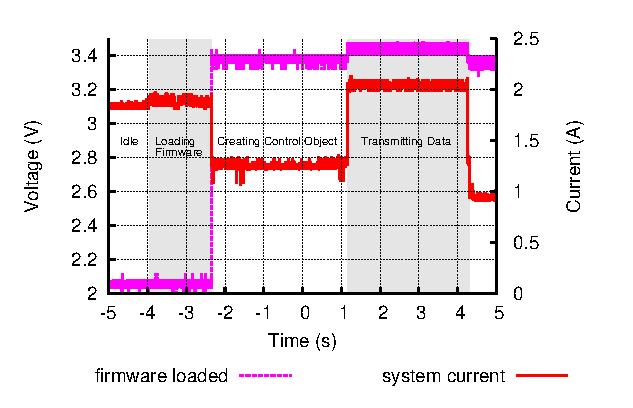
\includegraphics[width=0.98\columnwidth]{usrp_e100_run/usrp_e100_run}
	\caption{USRP E100 power profile. E100 runs a full embedded Linux
platform, making cold-boot an untenable comparison. Rather we show the timing
from an idle, booted system to load a firmware image (configure the FPGA) and
send the data.  The firmware loaded signal is recorded from a firmware loaded
pin. After configuration, the system idle power drops to
just under 1~A at 6~V.}
	\label{fig:usrp_e100}
\end{figure}

\begin{comment}
\subsection{Application Micro-Benchmarks}
To evaluate the \sdr system as a whole, we first compare the raw radio
performance against a current low-power radio: the TI CC2420. We then explore
the implementation of two recently proposed low-power protocols: A-MAC and
Glossy.

\subsubsection{Comparison with a CC2420}

\begin{figure}
	\centering
	\includegraphics[width=0.98\columnwidth]{R_inputPWR/R_inputPWR}
	\caption{Received signal strength vs. packet error rate (PER) of \sdr. If
the received signal strength is $>$~-90~dBm, then we have a PER of $<$~1\%. As a
comparison, the TI~CC2420 radio achieves a PER of $<$~1\% at a received signal
strength $>$~-90~dBm. This indicates that our receiver is competitive with
current state of the art radio hardware, but not yet optimal.}
	\label{fig:R_per}
\end{figure}

% Is this assertion from the epic paper too strong?
The CC2420 radio - and its successor the CC2520 - from Texas Instruments
represents the current standard in low-power wireless radios~\cite{epic}. In
Figure~\ref{fig:R_per} we evaluate the Packet Error Rate (PER) of \sdr as the
strength of the received signal degrades. We find \sdr able to perform
extremely well for strong signals ($>$-90~dBm), with a PER of $<1\%$. As the
signal degrades beyond -90~dBm, however, \sdr loses ground to the CC2420,
which is able to hold the PER below $<1\%$ beyond -90~dBm.

We argue then that \sdr is a very capable radio, useful for the development
and evaluation of various low-power MAC protocols as shown in the following
sections. However, we also recognize that there is still work to be done
before software radios can fully replicate the receive quality of fixed
function radio devices and replace them in general deployments.

\subsubsection{Validating A-MAC Acknowledgments}
\begin{figure}
	\centering
	\includegraphics[width=0.45\textwidth]{ack_collision}
	\caption{A constructive ACK collision observed and decoded. CH1
(yellow) is the RX baseband signal. CH3 (purple) is the RSSI. CH2 (blue) and
CH4 (green) are the TX baseband signals of the two colliding ACKs. The
slightly offset carrier frequencies of CH2 and CH4 interact to form the
envelope modulation on the received baseband signal.  Without automatic gain
control, varying signal strength resulting from the envelope severely hinders
the receiver's ability to successfully decode the signal.}
	\label{fig:ack_collision}
\end{figure}

Previous research~\cite{2010.amac} proposed using ACK frames to design a
receiver initiated MAC protocol. Unfortunately that work was built upon the
fixed function CC2420 radio, which did not allow sufficient flexibility to
fully realize the protocol. We investigate the A-MAC protocol's colliding ACK
primitive on the \sdr platform, both to validate the original A-MAC protocol
and as a demonstration of the capabilities of the \sdr platform.


In A-MAC we can assume two nodes transmit the same packet $d(t)$ with carrier
frequencies $f_1$ and $f_1 + \Delta f$ at the same time.
The received RF-signal $r(t)$ then is achieved by summing the $d(t)$
modulated with each carrier frequency $f_1$ and $f_1 + \Delta f$:
\[r(t) = d(t) \times \left[ cos(2\pi \times f_1 \times t ) + cos(2\pi \times(f_1 + \Delta f)\times t) \right] \]
This equation can be simplified using the sum-to-product identity:
\[r(t) = d(t) \times \left[ cos(2\pi \times \tfrac{2f_1 + \Delta f}{2} \times t) \times cos(2\pi \times \tfrac{\Delta f}{2} \times t) \right] \]
And if $2f_1 \gg \Delta f$, we can approximate $r(t)$:
\[r(t) \approx d(t) \times \left[ cos(2\pi \times f_1 \times t) \times cos(2\pi \times \tfrac{\Delta f}{2} \times t) \right] \]
Thus by down conversion, the received baseband signal $r_B(t)$ can be expressed
as:
\[r_B(t) \approx d(t) \times cos(2\pi \times \tfrac{\Delta f}{2} \times t)\]
The takeaway here is the existence of an envelope frequency of $\Delta f/2$
that encompasses the received ACKs.  Figure~\ref{fig:ack_collision} shows an
example of a packet collision and the resultant envelope. The envelope
introduces {\em local minimums} to the received signal.  These are important
as the signal amplitude is attenuated during a local minimum, which may cause
the receiver to incorrectly decode the signal. Local minimums occur while the
following condition is met:
\[2\pi \times \tfrac{\Delta f}{2} \times t = \tfrac{\pi}{2} \times n \hspace{10 pt} n \in N\]
Dutta et. al. measured the acknowledgment reception rate (ARR) for
varying numbers of concurrently transmitting neighbors. Their result shows the
worst case ARR could be as high as 97\%~\cite{dutta:ack_collision}.

As an example of radio optimization enabled by \sdr unavailable in either
highly latent SDRs or fixed function radios, we explore the effect of various
automatic gain control (AGC) methods on packet reception rate from two
concurrent transmitters. Automatic gain control attempts to detect varying
strength signals and dynamically adapt the amplitude of the raw RF signal for
further processing. The available resolution of AGC is highly dependent on the
latency of the AGC controller.  Highly latent devices such as the USRP
platform can only perform AGC on a {\em per-packet} basis whereas \sdr is
capable of performing AGC on a {\em fixed-latency} basis. In addition to latency
issues, many SDR platforms do not provide a sufficient degree of introspection
into the RF frontend to allow for fine-grained AGC, relying instead on metrics
such as RSSI.

\begin{figure}
	\centering
	\includegraphics[width=0.98\columnwidth]{R_df/R_df}
    \caption{Reception rate versus carrier frequency separation of two
concurrent transmitters with a fixed packet length (60 bytes). The period of
the beat frequency of the enveloping modulation is $T=\frac{2}{{\Delta}f}$.
For small $\Delta f$, this period is sufficiently long that continuous AGC is
able to correct for the varying signal strength (compare
Figure~\ref{fig:ack_collision} CH3). As $\Delta f$ grows, the beat
period shortens until it is too fast for continuous AGC to keep up. At this
point, however, the minima are sufficiently narrow to only obscure a few chips
and the spreading built into 802.15.4 recovers the missing information. The
continuous AGC's attempt to follow the high-frequency minima account for for
the slightly worse performance of continuous AGC at higher $\Delta f$s.}
	\label{fig:R_df}
\end{figure}

Traditional AGC in commodity radios latches a gain value upon receiving the
Start of Frame Delimiter (SFD). This AGC loop is sufficient if the amplitude
of a signal is constant over the entire packet. However, if multiple nodes
transmit concurrently, a radio with SFD-latched AGC may experience a changing
signal amplitude over time from the envelope module as seen
in Figure~\ref{fig:ack_collision}. We implemented both SFD-latched AGC and a
continuous AGC in \sdr. Table~\ref{tab:ARR_versus_agc_mode} summarizes the
results of a basic comparison. Continuous AGC provides a slight improvement in
acknowledgment reception rate (ARR) over SFD-latched AGC.

Further experimentation with AGC revealed that the properties of each AGC
method rely heavily on the degree of separation between the two carrier waves.
Figure~\ref{fig:R_df} plots the reception rate of concurrently transmitted 
packets against varying differences in the two transmitting carrier wave
frequncies. Recall that the period of the beat frequency of the modulating
envelope is given by $T=\frac{2}{\Delta f}$. For lower values of $\Delta f$,
this means the period of envelope beats will be relatively long and the
continuous AGC is able to adapt and correct for the variation in signal
strength. As $\Delta f$ increases, however, the local minima from the
envelope wave increase in frequency (while decreasing in length). Eventually
the continuous AGC cannot adapt fast enough to the varying signal strength
imposed by the envelop. At this point however, the period of the minima is
sufficiently short that only individual {\em chips} of the transmitted data
are lost. The 802.15.4 protocol employs a spreading technique such that 4 bits
are data are composed into 1 symbol made up of 32 {\em chips}. The redundancy
supplied by the spreading means that once the beat frequency of the envelope
is too high to correct via AGC, only a few {\em chips} of the symbol are
dropped, allowing the symbol as a whole to be correctly decoded. This
phenomena explains the observed upward trend of the SFD-Latch AGC as $\Delta
f$ increases.

As $\Delta f$ grows sufficiently large, the frequnecy of the minima begins to
approach and ultimately surpass the speed of the continuous AGC control loop.
The loop delay of the continuous AGC calculation then causes the actual gain
to be applied to the incoming signal too late. The extra strength oscillation
imposed by the late gain adaptation accounts for the $1\realtilde2\%$ worse
performance of continuous AGC versus the latched AGC for high $\Delta f$s.

% pull some more of the text from the very end of orig sdr eval

\subsubsection{Validating Glossy Broadcast Collisions}
Thus far we have focused exclusively on ACK collisions, which are relatively
short packets (11 bytes). In Glossy, the authors observed that the same
constructive ACK-collision optimization could be applied to broadcast packets.
We implemented a n\"ive broadcast, each node flooding the network. In this
broadcast scheme, the packet forwarding time is controlled precisely. This
allows multiple forwarded packets to (ideally) interfere constructively. It is
important to note here that unlike the short, fixed-length ACK packets, the
forwarded broadcast packets may be of arbitrary length and possibly quite
long. We can infer from the previous work that {\em reception rate should drop
if more envelopes exist during a given packet}.

Given two nodes with a fixed but slightly different carrier frequency, we
measured the reception rate across different packet lengths.
Figure~\ref{fig:R_length} shows our expected trend: as the packet length
increases, the reception rate decreases. The reception rate is derived from
the number of packets with a successfully decoded CRC value over 30000
transmissions. If any symbol in the packet is incorrectly decoded, that packet
will fail the CRC check.

\begin{figure*}
	\centering
		\subfigure[RF frequencies separate by 33.3~KHz]{
			\includegraphics[width=0.45\textwidth]{../figs/R_length/R_length_hdf}
			\label{fig:R_length_hdf}
		}
		\subfigure[RF frequencies separate $<$1~KHz]{
			\includegraphics[width=0.45\textwidth]{../figs/R_length/R_length_ldf}
			\label{fig:R_length_ldf}
		}
	\caption{
Reception rate of constructively interfering packet collisions with the
transmitter at two slightly different carrier frequencies. Both transmitters
send the exact same message, at the same time. Figure
\subref{fig:R_length_hdf} shows the result when the transmitters are separated
by 33.3~kHz, while Figure \subref{fig:R_length_ldf} depicts the case of the
transmitters separated by $<$1~kHz. In both cases, the longer the packets,
the lower the reception rate as we get more beats in a single packet. This
leads to a lower signal amplitude, and thus potential for decoding errors. To
mitigate this, the AGC can be held constant after latching it at the SFD
detection, or it can continuously updated over the whole packet length.  For
small carrier frequency offsets (Figure \subref{fig:R_length_ldf})
continuously updating the AGC improves the reception rate by 2$\sim$6\%.}
	\label{fig:R_length}
\end{figure*}
\end{comment}

